\chapterA{Evaluación de parámetros físicos del diseño}
\section{Parámetros}
\textbf{Área (tamaño).} Tamaño de silicio ($cm^{2}$ o $mm^{2}$) necesarios para implementar una determinada aplicación. Depende de la arquitectura del circuito y de la tecnología empleada para su fabricación. Si no tenemos el layout del circuito podemos estimarlo con un número de puertas NAND equivalente.\\
\textbf{Velocidad (tiempo).} La velocidad de un circuito se corresponde con el tiempo necesario para realizar una determinada función, normalmente este concepto se calcula sobre el peor caso posible. Siempre es deseable que el circuito sea lo más rápido posible, pero casi siempre para conseguirlo se necesita un diseño más sofisticado, lo que puede implicar un mayor área de silicio y/o un mayor consumo de energía. La velocidad de un circuito está directamente relacionada con la frecuencia de reloj, pero no es verdad que una mayor frecuencia de reloj garantice que el resultado se obtenga en menos tiempo. Tendremos que evaluar a qué frecuencia puede trabajar el circuito, cuántas operaciones puede realizar por unidad de tiempo y si funcionará correctamente a la frecuencia de reloj exigida.\\
\textbf{Potencia (energía).} La potencia hace referencia a la energía consumida por el circuito al realizar las operaciones para las cuales fue diseñado. En todos aquellos circuitos diseñados para dispositivos móviles la reducción del consumo de potencia es la prioridad. Antes de su fabricación el circuito puede ser rediseñado para cumplir los requisitos de consumo. Un mismo diseño consume menos en tecnologías. La temperatura que alcanza un circuito está directamente relacionada con el consumo de energía. Cuanto mas dure la batería de un circuito, menor será el impacto medioambiental. \\
\textbf{Coste.} El diseño de un circuito digital es rara vez un objetivo en sí mismo. Se trata de una actividad económica y el coste es un importante factor, si no el decisivo.
En el coste final del circuito influyen:
\begin{itemize}
    \item El coste de desarrollo (diseño)
    \item El coste de producción (diseño y fabricación)
    \item El tiempo de salida al mercado (comercialización)
\end{itemize}


La importancia de la evaluación es:
\begin{itemize}
    \item Conseguir diseños más rápidos, con mayor capacidad de procesamiento y reducción en la cantidad de recursos hardware para realizar las mismas operaciones.
    \item Diseños más pequeños, menor coste de fabricación, menor posibilidad de errores físicos durante la fabricación y aumentar la capacidad de integración.
    \item Diseños más eficientes energéticamente, con menor huella de $CO_{2}$, mayor duración de la batería y menor coste de operación.
\end{itemize}

\section{Análisis estático de tiempos (STA)}
El análisis de la temporización de un circuito recibe el nombre de \textbf{Análisis Estático de Tiempos (STA).} Determina si el circuito satisface los requisitos de temporización impuestos por el reloj.
\\ Para este análisis debemos calcular el retardo de todos los caminos del circuito y determinar si su valor es mayor o menor que el valor límite impuesto por la señal de reloj. Si es mayor el retardo, entonces se produce una violación del timing. Si es menor, entonces el camino más lento establece la frecuencia máxima del reloj.

\subsection{Retardo de camino}
Es la suma de los retardos de la lógica y conexiones desde:
\begin{itemize}
    \item Las entradas primarias hasta las salidas primarias para todos los posibles caminos combinacionales.
    \item Las entradas primarias hasta los elementos de memoria.
    \item Los elementos de memoria hasta las salidas primarias.
    \item Desde los elementos de memoria hasta los elementos de memoria.
\end{itemize}
\textcolor{blue}{Retardo de lógica}: retardo de las puertas o elementos lógicos del circuito.
\begin{itemize}
    \item Combinacionales. OR, AND, sumadores, decodificadores\dots
    \item Secuenciales: FF, contadores, registros, memorias \dots
\end{itemize}
\textcolor{blue}{Retardo de conexión}: todas las conexiones del circuito tienen un retardo.

\subsection{Modelado retardo: timing arcs}
Combinacional: retardo desde cualquier entrada a cualquiera de sus salidas. Secuencial: retardo desde el pin del reloj hasta cualquiera de sus salidas, a este tiempo se le conoce como Clk-2-Q. Conexiones: retardo desde el pin de salida hasta cada uno de sus destinos.
\section{Cálculo de tiempo de propagación}
Se suman todos los retardos de la lógica y las conexiones para todos los caminos del circuito  combinacional. Depende del camino, hay tantos tiempos como caminos. Se usa el valor del camino más lento, conocido como \textbf{camino crítico.}
\subsection{Funcionamiento síncrono}
Si en el sistema hay elementos de memoria debe existir un reloj. El reloj determina cuándo se actualiza el estado de los elementos de memoria del sistema.\\
La hipótesis de funcionamiento síncrono obliga a que la diferencia en tiempo entre dos flancos consecutivos (positivos o negativos los dos) sea superior al tiempo necesario para que los valores de las entradas de los registros sean estables.
\subsection{Definiciones}
\noindent\textbf{Tiempo de set-up:} tiempo mínimo que la entrada debe permanecer antes del suceso del reloj.\\
\textbf{Tiempo de hold:} tiempo mínimo que la entrada debe permanecer estable después del suceso del reloj.\\
\textbf{Tiempo de propagación del registro:} tiempo que tarda en propagarse el dato desde la entrada hasta la salida del registro cuando ocurre el flanco activo de reloj.\\
\textbf{Tiempo de propagación combinacional:} tiempo desde que cambian las entradas del circuito combinacional hasta que se produce un cambio en las salidas. Depende del camino. Se usa el valor del camino crítico.\\
\begin{multicols}{2}
    \begin{figure}[H]
        \centering
        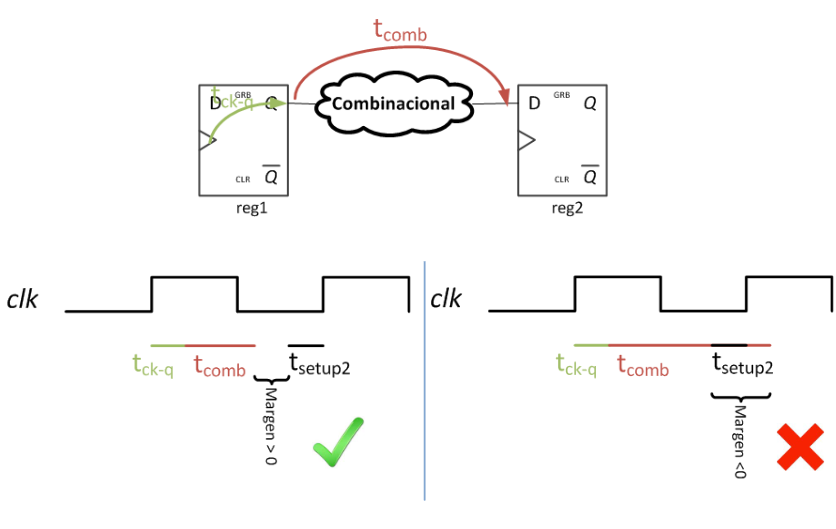
\includegraphics[width=0.4\textwidth]{images/Tema_2/Margen_setup.PNG}
        \caption{Margen de setup}
    \end{figure}
    \vfill
    \null
    \begin{figure}[H]
        \centering
        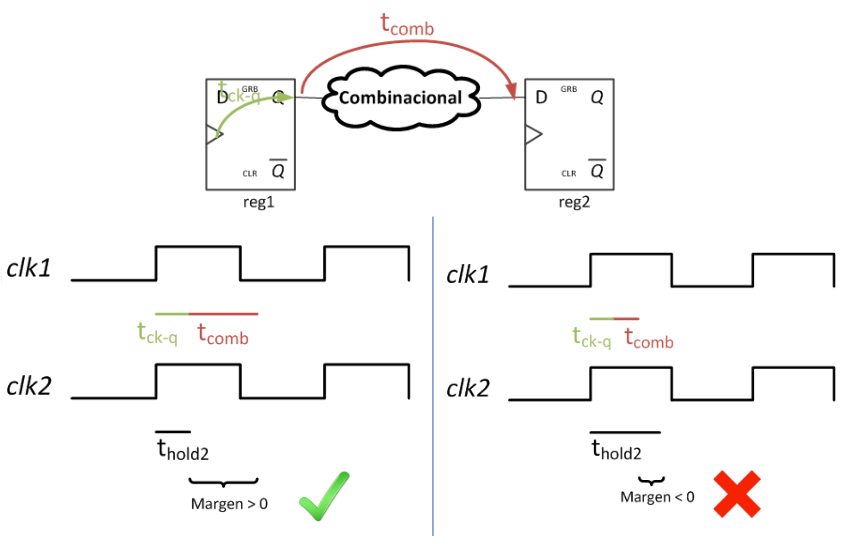
\includegraphics[width=0.4\textwidth]{images/Tema_2/Margen_hold.PNG}
        \caption{Margen de setup}
    \end{figure}
\end{multicols}
\subsection{Cálculo de tiempo de set-up y hold}
Sin considerar el clock skew y el clock jitter:
\[
    Margen\; setup = t_{clk}- \left(t_{clk_q} +t_{comb} + t_{setup}\right)
\]
\[
    Margen \; hold = t_{clk_q} + t_{comb} + t_{hold}
\]
Margen negativo $\rightarrow$ \textcolor{red}{error de temporización}
\begin{figure}[H]
    \centering
    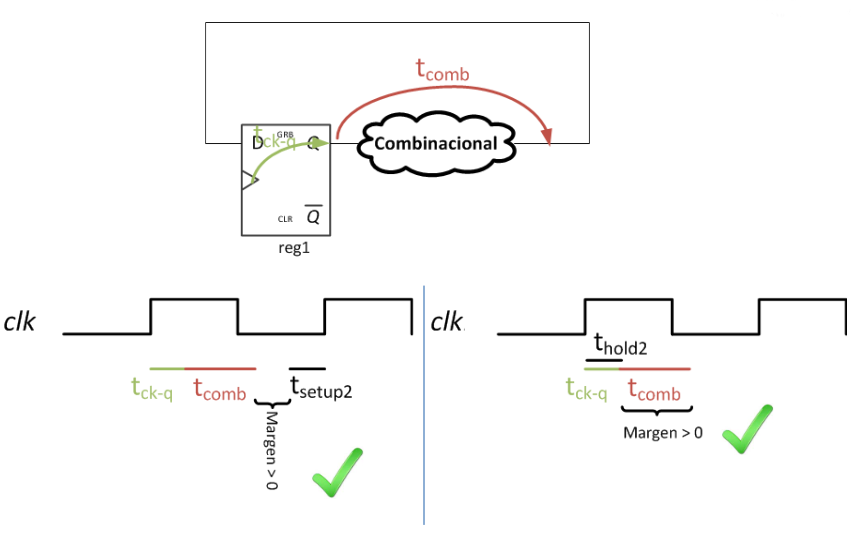
\includegraphics[width=0.8\textwidth]{images/Tema_2/Circ_retroalimentado.PNG}
    \caption{Circuito retroalimentado}
\end{figure}

\subsection{Metaestabilidad}
Consiste en una indecisión prolongada en el comportamiento lógico del  biestable al intentar almacenar uno de sus dos estados estables.
Ocurre si existe una violación de setup o de hold. Mientras ese biestable permanezca en metaestabilidad, sus señales de salida están indefinidas a nivel lógico.
\subsection{Clock skew}
El sesgo del reloj es un fenómeno que ocurre en los circuitos secuenciales cuando el reloj no llega al mismo tiempo a todos los componentes de memoria. Puede deberse a la longitud del cable, variaciones de temperatura, capacidades parásitas, imperfecciones del silicio, etc.
Cuando el tiempo de ciclo es pequeño, este problema se convierte en uno de los más importantes a la hora de diseñar el circuito.\\
Hay dos tipos de clock skew:
\begin{itemize}
    \item\textbf{Positive skew:} el registro que transmite recibe el reloj antes que el registro que recibe.
    \item\textbf{Negative skew:} el registro que transmite recibe el reloj después que el registro que recibe.
\end{itemize}
\[
    skew=t_{dest}-t_{orig}
\]

\subsection{Clock jitter}
El jitter es una modificación no deseada en la periodicidad del reloj. En otras palabras, es la variación de los flancos de reloj respecto de su posición ideal en el tiempo.
Tiene orígenes muy variados, variaciones en la fabricación de los osciladores, variaciones de temperatura etc.\\
Se especifica de tres maneras:
\begin{itemize}
    \item\textbf{Jitter absoluto:} diferencia entre la posición real del flanco de reloj y su posición ideal.
    \item\textbf{Jitter periódico:} diferencia entre el periodo real del reloj y el periodo ideal. Es el más importante a efectos de STA
    \item\textbf{Jitter ciclo-a-ciclo:} diferencia en la duración de dos periodos de reloj adyacentes
\end{itemize}

Es necesario tenerlo en cuenta en el análisis temporal del circuito porque puede acortar la duración del ciclo de reloj. Especificado como RMS(Root Mean Square) o valor pico-a-pico, se mide la duración media del ciclo sobre una muestra y se obtiene su desviación estándar.

\subsection{Cálculo de tiempo de setup y hold}
Considerando el clock skew y el clock jitter
\[
    Margen\; setup = t_{clk} + skew - \left(t_{clk\_q} + t_{comb} + t_{setup} + jitter\right)
\]
\[
    Margen\; hold = t_{clk\_q} + t_{comb} - \left(skew + jitter + t_{hold}\right)
\]
Margen negativo $\rightarrow$ \textcolor{red}{error de temporización}
\[
    t_{clk} + skew > \left(t_{clk\_q} + t_{comb} + t_{setup} + jitter\right)
\]
\[
    t_{clk} > \left(t_{clk\_q} + t_{comb} + t_{setup} + jitter\right) -skew
\]

\subsection{Falso camino crítico}
Parece el camino más lento del circuito pero en realidad no lo es, no propaga una transición. Los diseños que comparten lógica para distintos cálculos son susceptibles de tener falsos caminos.

\section{Segmentación}
Dividir un circuito en etapas usando registros. Las salidas de los registros de una etapa proporcionan las entradas de la siguiente etapa. Todas las etapas operan concurrentemente.
\begin{figure}[H]
    \centering
    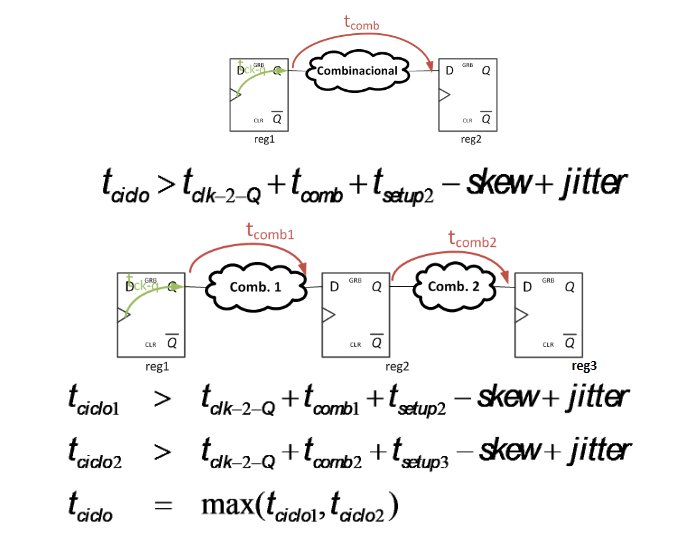
\includegraphics[width=0.7\textwidth]{images/Tema_2/segmentacion2.PNG}
    \caption{tiempo de ciclo}
\end{figure}

\subsection{Rendimiento}
\textbf{Latencia:} tiempo transcurrido para obtener un nuevo resultado a la salida del circuito desde su entrada en este.
\[
    L = n*t_{ciclo}
\]
\textbf{Intervalo de inicialización (Throughput):} tasa de entrada de nuevos datos en el sistema por unidad de tiempo.
\[
    T = \frac{1}{t_{ciclo}}
\]

\section{Comportamiento dinámico}
La simulación lógica no mide retardos. Los retardos se miden en la Simulación Post-Place \& Route. La herramienta calcula el retardo de todos los caminos, el más lento, llamado camino crítico, es el que define el retardo del circuito. El retardo de los distintos caminos del circuito puede originar errores funcionales.

\subsection{Azares y glitches}
El retardo de propagación de un circuito se define como el tiempo necesario para obtener un valor de salida válido. Los azares o riesgos son las posibles fluctuaciones de la señal de salida antes de alcanzar su valor final:
\begin{itemize}
    \item Riesgo estático
    \item Riesgo dinámico
\end{itemize}
Estas fluctuaciones pueden ser uno o varios pulsos no deseados que reciben el nombre de glitches.

\subsection{Riesgos estáticos}
Un determinado cambio en la entrada produce un glitch en la salida cuando no debería producirse ningún cambio. Se deben a la existencia de distintos caminos que convergen hacia la salida con diferente retardo.

\subsection{Riesgos dinámicos}
La salida debe cambiar pero el cambio no es directo sino con fluctuaciones. Suelen producirse en circuitos con riesgo estático y un nivel más de puertas.

\subsection{Análisis de consumo}
Existen distintas métricas: potencia (temperatura) y  energía (duración de la batería).
Existe también el consumo estático y dinámico.

\subsection{Consumo estático}
Consumo de los bloques de circuito cuando no hay transiciones en las señales de entrada.
\[
    P_{static} = V_{dd} * I_{static}
\]
Donde:
\begin{itemize}
    \item $I_{static}$ es la corriente estática
    \item $V_{dd}$ es la tensión de alimentación
\end{itemize}

$I_{static}$ depende de la corriente de fuga de los transistores, la tensión de alimentación y la temperatura.

\subsection{Consumo dinámico}
Consumo de los bloques del circuito cuando hay transiciones en las señales de entrada.
\[
    P = \frac{1}{2}*C_{load}*V_{dd}^{2} * f * t
\]
Donde:
\begin{itemize}
    \item $C_{load}$ es la capacidad de carga
    \item $V_{dd}$ es la tensión de alimentación
    \item $f$ es la frecuencia del reloj
    \item $t$ es la tasa de actividad de la puerta
\end{itemize}
